\documentclass[conference]{IEEEtran}
\IEEEoverridecommandlockouts
\usepackage{cite}
\usepackage{amsmath,amssymb,amsfonts}
\usepackage{algorithmic}
\usepackage{hyperref}
\usepackage{graphicx}
\usepackage{textcomp}
\usepackage{xcolor}
\hypersetup{
    colorlinks=true,
    linkcolor=red}
\def\BibTeX{{\rm B\kern-.05em{\sc i\kern-.025em b}\kern-.08em
    T\kern-.1667em\lower.7ex\hbox{E}\kern-.125emX}}
\begin{document}

\title{Visual Explanations for Deep Neural Nets}

\author{\IEEEauthorblockN{Siddhant Midha}
\IEEEauthorblockA{\textit{Sophomore, Electrical Engg.} \\
\textit{IIT Bombay}\\
\href{mailto:siddhantm@iitb.ac.in}{\texttt{siddhantm@iitb.ac.in}}}
\and
\IEEEauthorblockN{Prateek Garg}
\IEEEauthorblockA{\textit{Sophomore, Electrical Engg.} \\
\textit{IIT Bombay}\\
\href{mailto:prateekgarg@ee.iitb.ac.in}{\texttt{prateekgarg@ee.iitb.ac.in}}}}

\maketitle

\begin{abstract}
With the evolution of Machine Learning and Deep Learning, we have come up with more and more complex networks which perform very well on various tasks. Through this development, one caveat remains. Increasing complexity of the network leads to decreasing interpretability. In this report, we review few such methods and implement them. 
\end{abstract}

\begin{IEEEkeywords}
Saliency, Occlusion Sensitivity, Class Activation Maps 
\end{IEEEkeywords}

\section{Introduction}
There are two broad areas where an interpretation of the workings of neural networks proves useful - in the researcher's understanding, and as a proof of working to the stakeholders. We survey methods that facilitate the visualisation of the network, namely \textbf{Saliency Maps}, \textbf{Occlusion Sensitivity}, \textbf{Class Activation Maps} and \textbf{Deconvolution}. For some more insight, we also plot the learned \textbf{feature maps} at different locations in the network. The code can be found \href{https://github.com/prateekgargX/Visualizing-Neural-Networks}{here}.
\section{Methods}
\subsection{Saliency Maps}

Let us review the method used by the authors in the original paper \cite{saliency}. Given a specific class, we query a Convolutional net about the spatial support of that particular class in the image. Formally, let $I$ be the image and let $\mathfrak{S}$ be the image space. We have the vectorizing function
\[L: \mathfrak{S} \to \mathbb{R}^{k\times1}\]
Thus $L(I)$ is the vectorized version of the image. With abuse of notation, let us denote this as $I$. Further for a class $c$ we have the score function
\[S_c: \mathbb{R}^{k\times1} \to \mathbb{R}\]
We consider the linear approximation,
\[S_c(I) \approx w_c^TI + b_c \text{ , where, } w_c^T \in \mathbb{R}^{k\times1}, b_c \in \mathbb{R}\]
Elementary calculus tells us that,
\[w_c = \frac{\delta S_c}{\delta I}\]
Now the authors claim that this matrix gives us an idea of which spatial locations the network is looking at while predicting the class to be $c$. This is backed by the intuition that the larger the derivative for a particular pixel, more the output is sensitive to that pixel. \\ 
Computationally, we arrive at the map as follows. Assume the input shape is $m \times n$. \begin{enumerate}
\item Firstly, the derivative vector is found by backpropagation.
\item Then, the vector is arranged in the same shape as the input image. Denote this $w_{i,j,c}$, where $i \in \{1,2 \dots m\}, j \in \{1,2 \dots n\}$ correspond to the x-y directions, and $c$ to the channel.
\item For all $i \in \{1,2 \dots m\}, j \in \{1,2 \dots n\}$, define $$\mathfrak{M}_{i,j} := max_c|w_{i,j,c}|$$
\end{enumerate}
Then, $\mathfrak{M}$ is the desired saliency map. \\
Positive gradients corresponds to the location of target object and Negative image gradients corresponds to the other objects of competing classes. 
Since for the final output we use absolute value, saliency maps are not class discriminative which means it cannot localize the category in the image.   

\subsection{Occlusion Sensitivity Maps}
To answer the question of whether the model is really identifying the object while classifying it, this \cite{occlusion} paper uses occlusion maps. This serves to be a coarser technique which does not require backpropagation at all. Here, we perform a systematic occlusion of the input image with an occluding object of some fixed size and monitor the output of the classifier. If and when some main features of the object being identified are occluded, the probability of classification of that object drops sharply. 

More formally, let our input image be $I \in \mathbb{R}^{m \times n \times c}$. Further, let $p \times q$ be the dimensions of the occlusion. We describe occlusion at the $(j,k)^{th}$ position as
\[I[j:j+p-1][k:k+q-1][:] \leftarrow 0\]
Finally, we prepare a map showing the probability of classification as a function of position of the occluder. This process is justified from natural intuition and it shows
that the visualization genuinely corresponds to the image structure that stimulates that feature map.
\subsection{Class Activation Map (CAM)}
A class activation map for a particular category indicates the discriminative image regions used by the CNN to identify that category. The authors of the paper \cite{CAM} define this in the following way. For a given image, let $f_k(x,y)$ represent the activation of unit $k$ in the last convolutional layer at spatial location $(x,y)$. Then, for the unit $k$ global average pooling is given as \[F_k := \sum_{(x,y)}f_k(x,y)\]
Now say we have the final softmax layer. Then, for some class $c$, the input to the softmax $S_c$ is 
\[S_c := \sum_k w_k^cF_k\]
Intuitively, the importance of $F_k$ in computing $S_c$ is given by the weight $w_k^c$. We have,
\begin{align}
S_c &= \sum_kw_k^c\left(\sum_{(x,y)}f_k(x,y)\right) \\ 
S_c &= \sum_{(x,y)}\sum_kw_k^cf_k(x,y) 
\end{align}
Then we define $\mathfrak{K}_c$, the class activation map for class $c$ as
\[\mathfrak{K}_c(x,y) := \sum_kw_k^cf_k(x,y)\]
Thus we claim that $\mathfrak{K}_c(x,y)$ indicates the importance of the activation at the spatial grid point $(x,y)$ leading to the activation of class $c$. This is because
\[S_c = \sum_{(x,y)}\mathfrak{K}_c(x,y)\]
Thus,The class activation map is simply a weighted linear sum of the presence of these visual patterns at different spatial locations. By simply upsampling the class activation map to the size of the input image, we can identify the image regions most relevant to the particular category


\section{Results}
\subsection{Saliency Maps}
We trained a simple classifier to distinguish between dogs and wolves, using a \cite{ResNet} backbone network, on top of which we put a $2048 \to 1$ linear layer followed by a sigmoid. For this, we used the \cite{dogvwolf} dataset on Kaggle. \\ Let us take a look at an image and its corresponding saliency.
\begin{figure}[H]
    \centering
    \subfigure[]{
    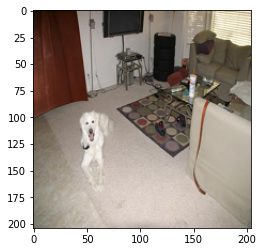
\includegraphics[width=.4\columnwidth]{2im.png}}
    \qquad
    \subfigure[]{
    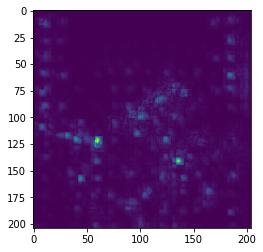
\includegraphics[width=.4\columnwidth]{2.png}}
    \caption[Short text]{Image and its Saliency Map}
\end{figure}
Through the previous result, we suspect a dependence on the backgroung. Now, we look at an image from the test set which was classified as a wolf.
\begin{figure}[H]
    \centering
    \subfigure[]{
    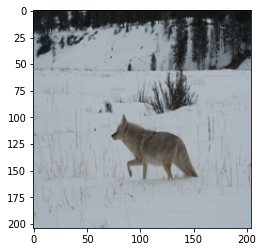
\includegraphics[width=.4\columnwidth]{3im.png}}
    \qquad
    \subfigure[]{
    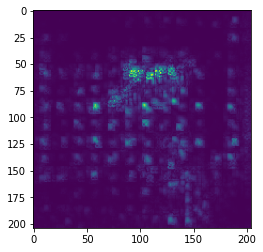
\includegraphics[width=.4\columnwidth]{3.png}}
    \caption[Short text]{Wolf  and its Saliency Map}
\end{figure}
We deliberately found an image of a dog with a white background, and fed it to the model to observe the following.
\begin{figure}[H]
    \centering
    \subfigure[]{
    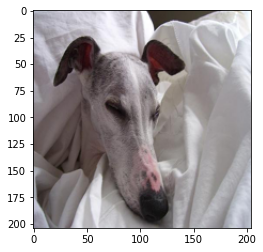
\includegraphics[width=.4\columnwidth]{4im.png}}
    \qquad
    \subfigure[]{
    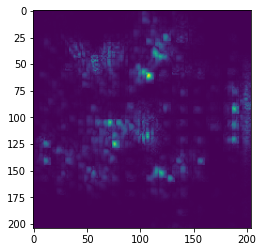
\includegraphics[width=.4\columnwidth]{4.png}}
    \caption[Short text]{A dog classified as a wolf}
\end{figure}
Thus, this technique enables us to comment on why certain classifications and particularly, some misclassifications are made.
\subsection{Occlusion Sensitivity Maps}
For testing occlusion sensitivity maps, we have used the model trained in the previous section. Results are given below. Note that the tuple in the caption is 
\[(\text{Size of occluder},\text{Stride of Occlusion})\]
Let us begin with looking at which areas of the image fire for classifying the image below as a wolf.
\begin{figure}[H]
    \centering
    \subfigure[]{
    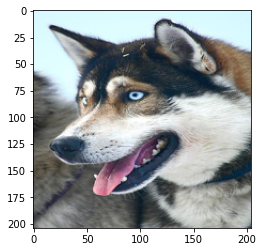
\includegraphics[width=.6\columnwidth]{occim1.png}}
    \qquad
    \subfigure[]{
    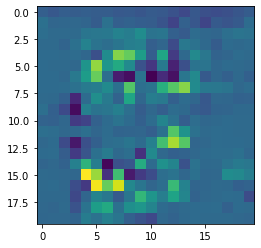
\includegraphics[width=.4\columnwidth]{occ1.png}}
    \qquad
    \subfigure[]{
    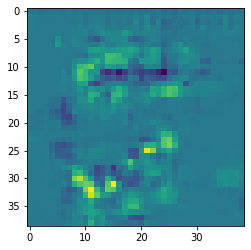
\includegraphics[width=.4\columnwidth]{occ1dash.png}}
    \caption[Short text]{Occlusion - (10,10) \& (10,5)}
\end{figure}
Let us look at another image of a dog with a man, and see which regions of the image indicate it is a dog.
\begin{figure}[H]
    \centering
    \subfigure[]{
    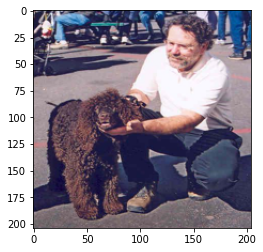
\includegraphics[width=.6\columnwidth]{occim2.png}}
    \qquad
    \subfigure[]{
    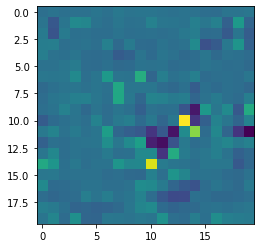
\includegraphics[width=.4\columnwidth]{occ2.png}}
    \qquad
    \subfigure[]{
    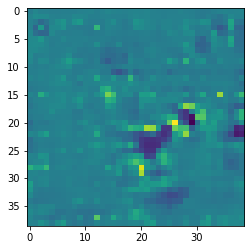
\includegraphics[width=.4\columnwidth]{occ2dash.png}}
    \caption[Short text]{Occlusion - (10,10) \& (10,5)}
\end{figure}
We can see that the model does not seem to be "looking" at the dog, and this is backed by the fact that probability of classification as a dog in this case is 67.96\%.
\subsection{Class Activation Maps}
We used pretrained network ResNet18 \cite{ResNet} from the \href{https://pytorch.org/}{torch} library. 
Since it already has a Global Average Pooling Layer after convolutional Layer, we directly create a hook at the forward pass. The heatmap superposed with image is created using \href{https://opencv.org/}{opencv}.
Other Networks which already have a GAP layer are Inception \cite{Inception}, SqueezeNet\cite{SqueezeNet}, and DensNet \cite{DensNet}.
\section*{Acknowledgment}

We thank the \texttt{Analytics Club, IITB} for giving us the opportunity to work on this project, and we are grateful to our mentor Saikiran for his help.

\begin{thebibliography}{00}
\bibitem{saliency} \href{https://arxiv.org/pdf/1312.6034.pdf}{Karen Simonyan, Andrea Vedaldi and Andrew Zisserman, ''Deep Inside Convolutional Networks: Visualising
Image Classification Models and Saliency Maps'' arXiv:1312.6034v2 [cs.CV] 19 Apr 2014}
\bibitem{occlusion} \href{https://arxiv.org/pdf/1311.2901.pdf}{Matthew D. Zeiler and Rob Fergus, ''Visualizing and Understanding Convolutional Networks'' arXiv:1311.2901v3 [cs.CV] 28 Nov 2013}
\bibitem{CAM} \href{http://cnnlocalization.csail.mit.edu/Zhou_Learning_Deep_Features_CVPR_2016_paper.pdf}{Bolei Zhou, Aditya Khosla, Agata Lapedriza, Aude Oliva, Antonio Torralba ''Learning Deep Features for Discriminative Localization'' Computer Science and Artificial Intelligence Laboratory, MIT}
\bibitem{ResNet} \href{https://arxiv.org/pdf/1512.03385.pdf}{Kaiming He, Xiangyu Zhang, Shaoqing Ren, Jian Sun, 'Deep Residual Learning for Image Recognition' arXiv:1512.03385 [cs.CV]}
\bibitem{Inception} \href{https://arxiv.org/pdf/1409.4842.pdf}{Wei Liu Et. al, Going deeper with convolutions arXiv:1409.4842v1 [cs.CV]}
\bibitem{SqueezeNet} \href{https://arxiv.org/pdf/1602.07360.pdf}{N. Iandola Et. al,'SqueezeNet: AlexNet-level accuracy with 50x fewer parameters and <0.5MB model size'	arXiv:1602.07360 [cs.CV]}
\bibitem{DensNet} \href{https://arxiv.org/pdf/1608.06993.pdf}{Huang Et. al,"Densely Connected Convolutional Networks" arXiv:1608.06993 [cs.CV]}
\end{thebibliography}
\end{document}
